\chapter{Implementation}\label{chap:5}
%EXPERIMENTAL RESULTS AND ANALYSIS
%
%
\section{Environment}
\section{Overview}
The system uses machine learning technique, known as decision tree algorithm for malware classification. The goal is classifying malware fast and decision tree algorithm is used to achieve that goal. Classification is a form of supervised learning, which requires training data, with known input/output, to form knowledge \cite{tonylee}. As shown in Figure \ref{fig:system_architec}, the system contains three following parts.

\begin{itemize}
\item First part: Read binary file to take meta data and input to database.
\item Second part: Manually cluster malware which load from database.
\item Third part: Use decision tree algorithm to classify malware.
\end{itemize}
\begin{figure}[h!]
\centering
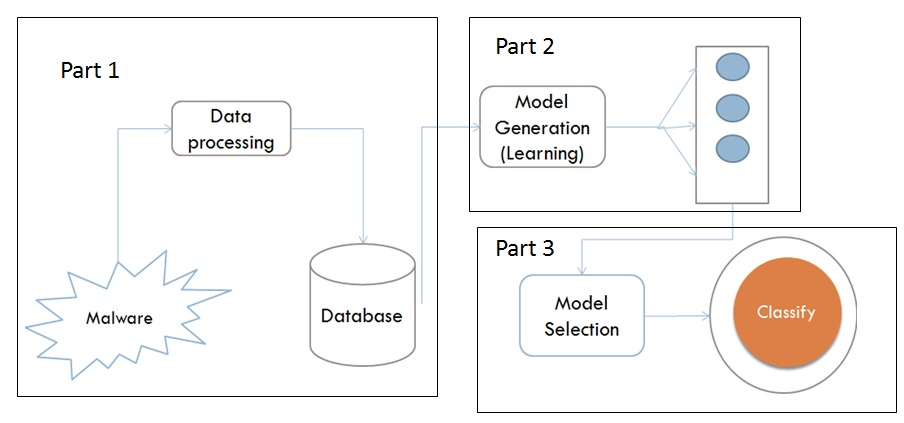
\includegraphics[width=1\textwidth]
{graph/system_architec1.jpg}
\caption{The system architecture.}
\label{fig:system_architec}
\end{figure}

A vast amount of malware need analyzing, and the system use database to store malware file's meta-data, to easily control a large number of data and to share them in the internet among web browsers.
The flow of data is shown in the Figure \ref{fig:system_architec}. Firstly, binary file meta-data are read, and all of the meta-data are input into database. In the second part, the system exports meta-data in database as the training data to create the decision tree for classifying malware. Finally	, the decision tree algorithm created in the second step is utilized to class  unknown malware into the different malware families. 
%CLASSFICATION BASE ON DECISION TREE
%
%
\section{Classification based on machine learning technique} 
\subsection{Meta-data}
In order to create a fast malware classification system, the system only use PE header's meta-data to classify malware. PE header includes meta-data of MS-DOS section, COFF file header, Optional header, and Section header.\\
There is a problem that PE file's meta data value is too large to detect unknown malwares which have meta-data's differences from the training data of the system. The meta-data of PE header file are indexed to give semantic information for malware classification. For example, normally \emph{ImageBase} field of PE header file has value of 400000h \cite{goppit}. The value of ImageBase of malware file in the system is 0 if it has 40000, and it is 1 if it has other value, ; in this research, that value is named as semantic value. This approach use all of PE file's meta-data, specifically \emph{HeaderFilesize}, \emph{AddressOfEntryPoint}, \emph{Sizeofsection}, \emph{Imagebase}, \emph{Numberofsection}, \emph{StackCommit}, \emph{SizeHeap Commit}, \emph{SizeImage}, \emph{Characteristics}. The semantic value of all malware file's meta-data is calculated.

\subsection{Create training data}
Virustotal is a service that analyzes malware and facilitates quick collection of viruses, worms, trojans, and all kinds of malware are detected by antivirus vendor such as Norton and Kaspersky \cite{virustotal}. This research applies virustotal service to take the name of malware provided by Kaspersky and uses it to  cluster malware into malware families with semantic information. 
Figure \ref{fig:clustering} indicates http post technique to automatically get name from virus total service and cluster malware into malware families which given in Figure \ref{fig:familymalware}.
\begin{figure}[h!]
\centering
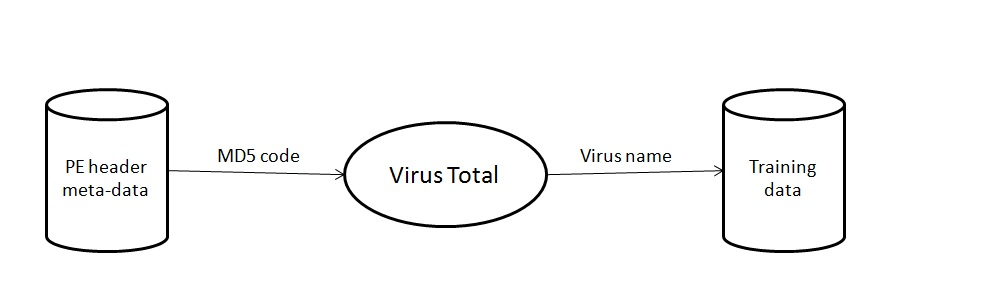
\includegraphics[width=1\textwidth]{graph/clustering.jpg}
\caption{Clustering method.}
\label{fig:clustering}
\end{figure}
\newline
\subsection{Classification}
\begin{figure}[h!]
\centering
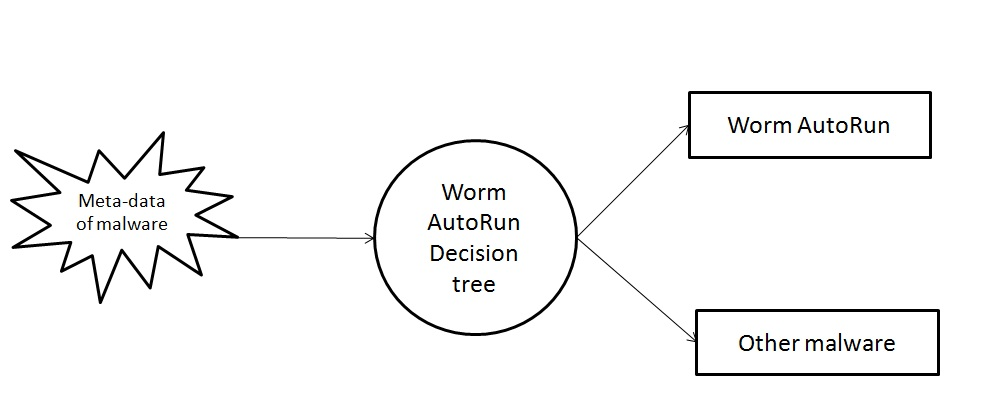
\includegraphics[width=1\textwidth]{graph/classificationdecision.jpg}
\caption{Worm autorun decision tree.}
\label{fig:classificationdecision}
\end{figure}

To make malware classification rapid and correct, decision tree algorithm is utilized. At that time, it is easy update a new malware family, the classification uses decision tree algorithm to determine each malware family. For example, based on training data from clustering part, six decision trees are created. In the worm autorun decision tree, shown is indicated in Figure \ref{fig:classificationdecision}.

Malware' meta-data are known as input data for each decision tree, and the the decision tree determines whether the malware belongs to worm autorun family or not. If the input malware belongs to worm autorun, malware classification shall detect which the family that malware is, otherwise it moves to the next decision tree. Lists of malware PE header file's meta-data are Magic, MajorLinkerVersion, MinorLinkerVersion, SizeOfCode, SizeOfInitializedData, SizeOfUninitializedData, AddressOfEntryPoint, BaseOfCode, BaseOfData, ImageBase, SectionAlignment, FileAlignment, MajorOperatingSystemVersion, MinorOperatingSystemVersion, MajorImageVersion, MinorImageVersion, MajorSubsystemVersion, MinorSubsystemVersion, Reserved1, SizeOfImage, SizeOfHeaders, CheckSum, Subsystem, DllCharacteristics, SizeOfStackReserve, SizeOfStackCommit, SizeOfHeapReserve, SizeOfHeapCommit, LoaderFlags, NumberOfRvaAndSizes, Machine, NumberOfSections, TimeDateStamp, PointerToSymbolTable, NumberOfSymbols, SizeOfOptionalHeader, Characteristics. The value of each field in PE header has semantics for decision tree algorithm if it is appeared at 10\% in malware training data. With this approach, the semantic value list of meta-data malware is made. For example, this is a list of meta-data created :1, 2, 6, 4, 0, 1, 1, 4, 0, 200, 4, 0, 0, 0, 4, 0, 0, 1.00E+00, 200, 0, 2, 0, 100000, 4000, 100000, 1000, 0, 10, 14c, 2, 1000, 8, 0, e0, 3, 818e. This is value before being computed :35328, 10b, 2, 0, 6200, 0, 200, b32e, b000, 9000, 400000, 1000, 200, 3, 0, 0, 0, 4, 0, 0, d000, 400, afe8, 2, 0, 1000, 1000, 10000, 0, 0, 10, 14c, 6, 0, 0, 0, e0, 10e. 
The malware classification part is shown in Figure \ref{fig:classification}. The training data from the malware clustering part is used to create the order of decision tree that makes malware classification system correct.
The decision tree is given as in Figure \ref{fig:decisiontreeworm}. When PE header's meta-data of malware is inputted into the worn autorun decision tree in order for determining unknown malware. Then, it decides whether it belongs to worm auto run family or not.\\
\begin{figure}[h!]
\centering
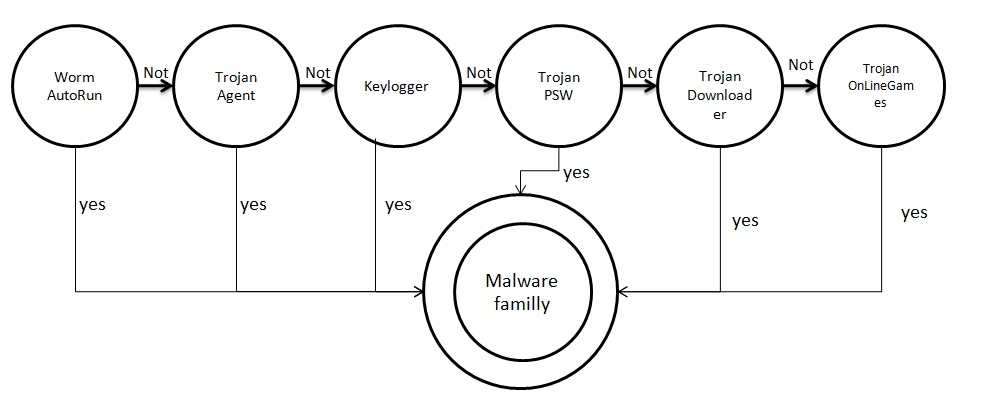
\includegraphics[width=1\textwidth]{graph/classification.jpg}
\caption{Malware classification system.}
\label{fig:classification}
\end{figure}
\begin{figure}[h!]
\centering
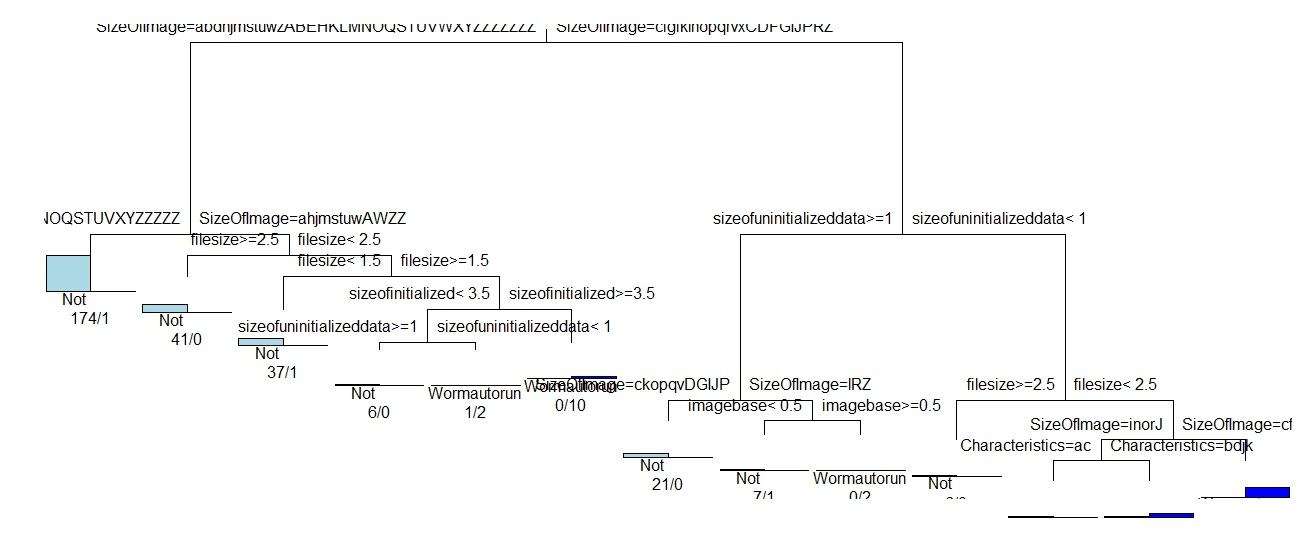
\includegraphics[width=1\textwidth]{graph/decisiontreeworm.jpg}
\caption{Worm autorun decision tree.}
\label{fig:decisiontreeworm}
\end{figure}
